\documentclass{article}
\usepackage[paperwidth=20cm, paperheight=6cm, margin = 0cm, top=0.5cm]{geometry}
\usepackage{amsmath}


\usepackage{pgf}
\usepackage{tikz}


\usetikzlibrary{arrows,automata}

\tikzstyle{source}  = [draw,circle,fill=black,thick,inner sep=0mm,minimum size=2mm]

\renewcommand{\vec}[1]{\boldsymbol{#1}}

\begin{document}
\begin{center}
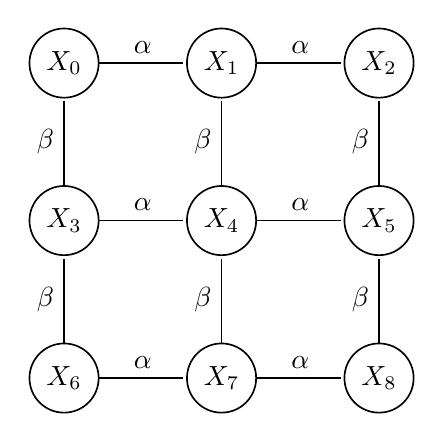
\begin{tikzpicture}[-,>=stealth',shorten >=1pt,auto,node distance=2cm,semithick]
                    
\node[state] (X1)               {$X_{6}$}; 
\node[state] (X2) [right of=X1] {$X_{7}$};                   
\node[state] (X3) [right of=X2] {$X_{8}$};                   

\node[state] (Y1) [above of=X1] {$X_{3}$}; 
\node[state] (Y2) [above of=X2] {$X_{4}$}; 
\node[state] (Y3) [above of=X3] {$X_{5}$}; 

\node[state] (Z1) [above of=Y1] {$X_{0}$}; 
\node[state] (Z2) [above of=Y2] {$X_{1}$}; 
\node[state] (Z3) [above of=Y3] {$X_{2}$}; 

	
\path
	(X1) edge node[above]{$\alpha$} (X2)
	(X2) edge node[above]{$\alpha$} (X3);
\path
	(Y1) edge node[above]{$\alpha$} (Y2)
	(Y2) edge node[above]{$\alpha$} (Y3);
\path
	(Z1) edge node[above]{$\alpha$} (Z2)
	(Z2) edge node[above]{$\alpha$} (Z3);

\path	
	(X1) edge node[left]{$\beta$} (Y1)
	(X2) edge node[left]{$\beta$} (Y2)
	(X3) edge node[left]{$\beta$} (Y3);
\path	
	(Y1) edge node[left]{$\beta$} (Z1)
	(Y2) edge node[left]{$\beta$} (Z2)
	(Y3) edge node[left]{$\beta$} (Z3);


\path	
	(Y1) edge (Z1)
	(Y2) edge (Z2)
	(Y3) edge (Z3);


\end{tikzpicture}
\end{center}

\end{document}
